% ========================================
%	Header einbinden
% ========================================

\documentclass[bibtotoc,titlepage]{scrartcl}

% Deutsche Spracheinstellungen
\usepackage[ngerman,german]{babel, varioref}
\usepackage[T1]{fontenc}
\usepackage[utf8]{inputenc}

%\usepackage{marvosym}

\usepackage{amsfonts}
\usepackage{amssymb}
\usepackage{amsmath}
\usepackage{amscd}
\usepackage{amstext}

\usepackage{longtable}

%\usepackage{bibgerm}

\usepackage{footnpag}

\usepackage{ifthen}                 %%% package for conditionals in TeX
\usepackage[amssymb]{SIunits}
%Für textumflossene Bilder und Tablellen
%\usepackage{floatflt} - veraltet

%Für Testzwecke aktivieren, zeigt labels und refs im Text an.
%\usepackage{showkeys}

% Abstand zwischen zwei Absätzen nach DIN (1,5 Zeilen)
% \setlength{\parskip}{1.5ex plus0.5ex minus0.5ex}

% Einrückung am Anfang eines neuen Absatzes nach DIN (keine)
%\setlength{\parindent}{0pt}

% Ränder definieren
% \setlength{\oddsidemargin}{0.3cm}
% \setlength{\textwidth}{15.6cm}

% bessere Bildunterschriften
%\usepackage[center]{caption2}


% Problemlösungen beim Umgang mit Gleitumgebungen
\usepackage{float}

% Nummeriert bis zur Strukturstufe 3 (also <section>, <subsection> und <subsubsection>)
%\setcounter{secnumdepth}{3}

% Führt das Inhaltsverzeichnis bis zur Strukturstufe 3
%\setcounter{tocdepth}{3}
\usepackage[version=3]{mhchem}
	\mhchemoptions{minus-sidebearing-left=0.06em, minus-sidebearing-right=0.11em}
\usepackage{exscale}

\newenvironment{dsm} {\begin{displaymath}} {\end{displaymath}}
\newenvironment{vars} {\begin{center}\scriptsize} {\normalsize \end{center}}


\newcommand {\en} {\varepsilon_0}               % Epsilon-Null aus der Elektrodynamik
\newcommand {\lap} {\; \mathbf{\Delta}}         % Laplace-Operator
\newcommand {\R} { \mathbb{R} }                 % Menge der reellen Zahlen
\newcommand {\e} { \ \mathbf{e} }               % Eulersche Zahl
\renewcommand {\i} { \mathbf{i} }               % komplexe Zahl i
\newcommand {\N} { \mathbb{N} }                 % Menge der nat. Zahlen
\newcommand {\C} { \mathbb{C} }                 % Menge der kompl. Zahlen
\newcommand {\Z} { \mathbb{Z} }                 % Menge der kompl. Zahlen
\newcommand {\limi}[1]{\lim_{#1 \rightarrow \infty}} % Limes unendlich
\newcommand {\sumi}[1]{\sum_{#1=0}^\infty}
\newcommand {\rot} {\; \mathrm{rot} \,}         % Rotation
\newcommand {\grad} {\; \mathrm{grad} \,}       % Gradient
\newcommand {\dive} {\; \mathrm{div} \,}        % Divergenz
\newcommand {\dx} {\; \mathrm{d} }              % Differential d
\newcommand {\cotanh} {\; \mathrm{cotanh} \,}   %Cotangenshyperbolicus
\newcommand {\asinh} {\; \mathrm{areasinh} \,}  %Area-Sinus-Hyp.
\newcommand {\acosh} {\; \mathrm{areacosh} \,}  %Area-Cosinus-H.
\newcommand {\atanh} {\; \mathrm{areatanh} \,}  %Area Tangens-H.
\newcommand {\acoth} {\; \mathrm{areacoth} \,}  % Area-cotangens
\newcommand {\Sp} {\; \mathrm{Sp} \,}
\newcommand {\mbe} {\stackrel{\text{!}}{=}}     %Must Be Equal
\newcommand{\qed} { \hfill $\square$\\}
\renewcommand{\i} {\imath}
\def\captionsngerman{\def\figurename{\textbf{Abb.}}}

%%%%%%%%%%%%%%%%%%%%%%%%%%%%%%%%%%%%%%%%%%%%%%%%%%%%%%%%%%%%%%%%%%%%%%%%%%%%
% SWITCH FOR PDFLATEX or LATEX
%%%%%%%%%%%%%%%%%%%%%%%%%%%%%%%%%%%%%%%%%%%%%%%%%%%%%%%%%%%%%%%%%%%%%%%%%%%%
%%%
\ifx\pdfoutput\undefined %%%%%%%%%%%%%%%%%%%%%%%%%%%%%%%%%%%%%%%%% LATEX %%%
%%%
\usepackage[dvips]{graphicx}       %%% graphics for dvips
\DeclareGraphicsExtensions{.eps,.ps}   %%% standard extension for included graphics
\usepackage[ps2pdf]{thumbpdf}      %%% thumbnails for ps2pdf
\usepackage[ps2pdf,                %%% hyper-references for ps2pdf
bookmarks=true,%                   %%% generate bookmarks ...
bookmarksnumbered=true,%           %%% ... with numbers
hypertexnames=false,%              %%% needed for correct links to figures !!!
breaklinks=true,%                  %%% breaks lines, but links are very small
linkbordercolor={0 0 1},%          %%% blue frames around links
pdfborder={0 0 112.0}]{hyperref}%  %%% border-width of frames
%                                      will be multiplied with 0.009 by ps2pdf
%
\hypersetup{ pdfauthor   = {Hannes Franke; Julius Tilly},
pdftitle    = {V301 Innenwiderstand und Leistungsanpassung}, pdfsubject  = {Protokoll FP}, pdfkeywords = {V301, Innenwiderstand, Leistungsanpassung},
pdfcreator  = {LaTeX with hyperref package}, pdfproducer = {dvips
+ ps2pdf} }
%%%
\else %%%%%%%%%%%%%%%%%%%%%%%%%%%%%%%%%%%%%%%%%%%%%%%%%%%%%%%%%% PDFLATEX %%%
%%%
\usepackage[pdftex]{graphicx}      %%% graphics for pdfLaTeX
\DeclareGraphicsExtensions{.pdf}   %%% standard extension for included graphics
\usepackage[pdftex]{thumbpdf}      %%% thumbnails for pdflatex
\usepackage[pdftex,                %%% hyper-references for pdflatex
bookmarks=true,%                   %%% generate bookmarks ...
bookmarksnumbered=true,%           %%% ... with numbers
hypertexnames=false,%              %%% needed for correct links to figures !!!
breaklinks=true,%                  %%% break links if exceeding a single line
linkbordercolor={0 0 1},
linktocpage]{hyperref} %%% blue frames around links
%                                  %%% pdfborder={0 0 1} is the default
\hypersetup{
pdftitle    = {V301 Innenwiderstand und Leistungsanpassung}, 
pdfsubject  = {Protokoll AP}, 
pdfkeywords = {V301, Innenwiderstand, Leistungsanpassung},
pdfsubject  = {Protokoll AP},
pdfkeywords = {V301, Innenwiderstand, Leistungsanpassung}}
%                                  %%% pdfcreator, pdfproducer,
%                                      and CreationDate are automatically set
%                                      by pdflatex !!!
\pdfadjustspacing=1                %%% force LaTeX-like character spacing
\usepackage{epstopdf}
%
\fi %%%%%%%%%%%%%%%%%%%%%%%%%%%%%%%%%%%%%%%%%%%%%%%%%%% END OF CONDITION %%%
%%%%%%%%%%%%%%%%%%%%%%%%%%%%%%%%%%%%%%%%%%%%%%%%%%%%%%%%%%%%%%%%%%%%%%%%%%%%
% seitliche Tabellen und Abbildungen
%\usepackage{rotating}
\usepackage{ae}
\usepackage{
  array,
  booktabs,
  dcolumn
}
\makeatletter 
  \renewenvironment{figure}[1][] {% 
    \ifthenelse{\equal{#1}{}}{% 
      \@float{figure} 
    }{% 
      \@float{figure}[#1]% 
    }% 
    \centering 
  }{% 
    \end@float 
  } 
  \makeatother 


  \makeatletter 
  \renewenvironment{table}[1][] {% 
    \ifthenelse{\equal{#1}{}}{% 
      \@float{table} 
    }{% 
      \@float{table}[#1]% 
    }% 
    \centering 
  }{% 
    \end@float 
  } 
  \makeatother 
%\usepackage{listings}
%\lstloadlanguages{[Visual]Basic}
%\allowdisplaybreaks[1]
%\usepackage{hycap}
%\usepackage{fancyunits}


% ========================================
%	Angaben für das Titelblatt
% ========================================

\title{Versuch 601 - Der Franck-Hertz-Versuch\\				% Titel des Versuchs 
\large TU Dortmund, Fakultät Physik\\ 
\normalsize Anfänger-Praktikum}

\author{Jan Adam\\			% Name Praktikumspartner A
{\small \href{jan.adam@tu-dortmund.de}{jan.adam@tu-dortmund.de}}	% Erzeugt interaktiven einen Link
\and						% um einen weiteren Author hinzuzfügen
Dimitrios Skodras\\					% Name Praktikumspartner B
{\small \href{dimitrios.skodras@tu-dortmund.de}{dimitrios.skodras@tu-dortmund.de}}		% Erzeugt interaktiven einen Link
}
\date{11.Juni 2013}				% Das Datum der Versuchsdurchführung

% ========================================
%	Das Dokument beginnt
% ========================================

\begin{document}

% ========================================
%	Titelblatt erzeugen
% ========================================

\maketitle					% Jetzt wird die Titelseite erzeugt
\thispagestyle{empty} 				% Weder Kopfzeile noch Fußzeile

% ========================================
%	Der Vorspann
% ========================================

%\newpage					% Wenn Verzeichnisse auf einer neuen Seite beginnen sollen
%\pagestyle{empty}				% Weder Kopf- noch Fußzeile für Verzeichnisse

\tableofcontents

%\newpage					% eine neue Seite
%\thispagestyle{empty}				% Weder Kopf- noch Fußzeile für Verzeichnisse
%\listoffigures					% Abbildungsverzeichnis

%\newpage					% eine neue Seite
%\thispagestyle{empty}				% Weder Kopf- noch Fußzeile für Verzeichnisse
%\listoftables					% Tabellenverzeichnis
\newpage					% eine neue Seite


% ========================================
%	Kapitel
% ========================================

%\section{Einleitung}				% Bei Bedarf

\section{Theorie}
\setcounter{page}{1}
Mit dem Franck-Hertz-Versuch konnten erstmals einige Aspekte der Bohrschen Postulate überprüft werden. In diesem Versuch werden Quecksilberatome durch Stöße mit Elektronen angeregt, so dass diese beim Zurückfallen in den Grundzustand Photonen mit der Differenzenergie zwischen den diskreten Elektronenhüllenniveaus erzeugen. Es treten dabei sowohl elastische, als auch inelastische Stöße auf.\\
Die Energiedifferenz des Elektrons nach dem unelastischen Stoß beträgt klassisch:
\begin{formel}[H]
$\Delta E = E_1-E_0 = \frac{1}{2}m_0v_{vor}^2 - \frac{1}{2}m_0v_{nach}^2$
\centering
\caption*{\small{$m_0$ - Ruhemasse des Elektrons, v - Geschwindigkeit vor/nach dem Stoß}}
\end{formel}
Den Betrag der Energie kann man mit der Gegenfeldmethode bestimmen.

Für den Franck-Hertz Versuch wird ein evakuierter Behälter mit einem Tröpfchen Quecksilber darin verwendet. Ein Teil des Quecksilbers verdampft  entsprechend der Gasdruckkurve, bis sich ein Gleichgewichtsdampfdruck einstellt. Der Druck und somit auch die Konzentration des Quecksilbers im Gefäß ist damit von der Temperatur abhängig. Diese kann mit einem Heizgenerator verändert werden.\\
Die freien Elektronen werden mittels Glühemission aus einem geheizten Wolframdraht erzeugt und über ein elektrisches Feld zur Gitteranode hin beschleunigt. Hinter der Gitteranode wird ein elektrisches Gegenfeld mit der Spannung $U_A$ angelegt, so dass nur Elektronen die Auffängereletrode erreichen können, die die Beziehung:
\begin{align}
\frac{m_o}{2} v^2_z \geq e_0 U_A
\label{eq_gegenfeld}
\end{align}
erfüllen. Dabei ist $v_z$ die Geschwindigkeitskomponente des Elektrons, die parallel zu den Feldlinien steht. Die an der Auffängerelektrode gemessene Stromstärke ist direkt proportional zur Anzahl der auftreffenden Elektronen und beschreibt daher, wieviele Elektronen die Beziehung \eqref{eq_gegenfeld} erfüllen.\\
Auf dem Weg zur Elektrode können die Elektronen mit den Quecksilberatomen zusammenstoßen. Ist die Energie der Elektronen gering, so finden elastische Stöße statt. Da die Masse des Hg-Atoms im Vergleich zum Elektron um mehrere Größenordnungen größer ist, ist die übertragene Energie nur gering, aber die Richtungsänderung des Elektrons kann massiv sein.\\
Hat das Elektron jedoch eine Energie erreicht, die größer oder gleich der Energiedifferenz zwischen dem Grundzustand und dem 1. angeregten Zustand
ist, so kann das Hg-Atom vom Elektron angeregt werden. Es übernimmt dabei die benötigte Energiedifferenz zwischen den beiden Zuständen vom Elektron $\Delta E=E_1-E_0$ und fällt nach etwa $10^{-8}$ Sekunden in seinen Grundzustand zurück, wobei es ein Photon mit der Energie 
\begin{align}
E_{Photon}=\Delta E = E_1-E_0 = h\nu
\label{eq_energie_phtoton}
\end{align}
emittiert.\\
Betrachtet man nun den Strom $I_A$ an der Auffängerelektrode in Abhängigkeit zur Beschleunigungsspannung $U_B$, so stellt man fest, dass der Strom mit wachsender Spannung zunächst steigt, dann jedoch auf ein Minimum abfällt und anschließend wieder steigt, bevor er erneut abfällt. Das Abfallen des Stromes erklärt sich dadurch, dass die Elektronen gerade genug Ernergie aus dem Elektrischen Feld aufgenommen haben, um das Hg-Atom anzuregen. Die Energie, die sie dabei abgeben, fehlt ihnen dann um das Gegenfeld zu überwinden. Erhöht man die Beschleunigungsspannung weiter, so erhalten die Elektronen nach dem Stoß wieder genug Energie, um die Gegenspannung zu überwinden. Ab einer bestimmten Spannung $U_B$ bekommt das Elektron nach dem ersten Stoß jedoch so viel Energie, dass es ein zweites Hg-Atom anregen kann und dann jedoch wieder an der Gegenspannung scheitert. Trägt man den Strom gegen die Spannung auf, so erhält man folgenden Graphen:
\begin{figure}[H]
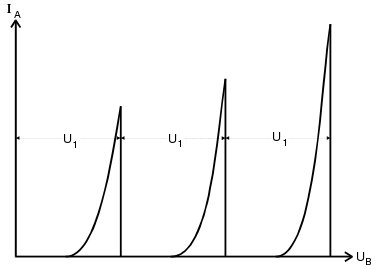
\includegraphics[width=0.7\textwidth]{pics/strom_spannung.jpeg}
\caption{Auffängerstrom gegen Beschleunigungsspannung (idealisiert)$^{[1]}$}
\label{pic_strom_spannung}
\end{figure}
Der Abstand zwischen den Peaks muss daher der Energiedifferenz zwischen dem Grundzustand und dem 1. angeregten Zustand des Hg-Atoms entsprechen:
\begin{align}
U_1:= \frac{1}{e_0}(E_1-E_0)
\end{align}
\subsection{Nebeneinflüsse}
Der Graph in Abbildung \ref{pic_strom_spannung} ist nur eine idealisierte Darstellung der Tatsächlichen Kurve. Es gibt noch drei Effekte, die das Bild des Graphen beeinflussen.
\subsubsection{Das Kontaktpotential}
\label{sec_kontakt}
Um bereits bei Zimmertemperatur viele Elektronen aus der Glühkathode austreten zu lassen, besteht diese aus einem Material mit einer geringen Austrittsarbeit als die Anode. Dies wirkt sich auf die Beschleunigungsspannung aus. Auf die austretenden Elektronen wirkt daher nur das effektive Potential
\begin{formel}[H]
\begin{align}
U_{eff}= U_B - \frac{1}{e_0}(\Phi_B-\Phi_G)
\label{eq_ionisation}
\end{align}
\caption*{\small{$\Phi_G$ - Austrittsarbeit Glühdrat, $\Phi_B$ - Austrittsarbeit Beschleunigungselektrode}}
\end{formel}
Die Franck-Hertz Kurve ist daher um den Wert
\begin{align}
K:=\frac{1}{e_0}(\Phi_B-\Phi_G)
\end{align}
nach rechts verschoben.
\subsubsection{Energie-Spektrum der Elektronen}
Den Aussagen der Quantenmechanik zufolge besitzten die Elektronen bereits im Metal eine Energie, die ungleich Null ist. Diese wird durch die Dirac-Verteilung beschrieben und muss der Energie $e_0 U_B$ hinzuaddiert werden.
Die Elektronen haben daher nicht alle die gleiche Energie und folglich sind die in Abbildung \ref{pic_strom_spannung} dargestellten scharf abfallende Kanten in Wahrheit etwas breiter verschmiert.\\
Auf die Geschwindigkeit der Elektronen wirkt sich ebenfalls aus, wenn diese noch nach dem Durchlaufen der Beschleunigungsspannung mit einem Hg-Atom kollidieren. Bei einem inelastischen Stoß können die Elektronen wie bereits erwähnt, teils sehr stark abgelenkt werden. Geschieht dies nach der Beschleunigung, so kann  es sein, dass die Geschwindigkeitskomponente parallel zu den Feldlinien nicht mehr groß genug ist, um das Feld zu überwinden.
\subsubsection{Der Dampfdruck}
\label{sec_dampfdruck}
Um gute Ergebnisse zu erhalten, müssen während des Durchlaufens der Beschleunigungsspannung hinreichend viele Hg-Atome getroffen werden können. Die mittlere freie Weglänge $\overline{w}$ sollte daher um einen Faktor 1000-4000 kleiner sein, als die Beschleunigungsstrecke a (hier etwa 1cm).\\

$\overline{w}$ berechnet sich zu:
\begin{formel}[H]
\begin{align}
\overline{w} = \frac{0,0029}{p_{sät}}
\label{eq_weglaenge}
\end{align}
\caption*{\small{$\overline{w}$ in [cm], $p_{sät}$ der Sättigungsgasdruck in [mbar]}}

\end{formel}
$p_{sät}$ lässt sich wiederum aus der Gasdruckkurve bestimmen. Diese lautet für Quecksilber:
\begin{align}
p_{sät} = 	e^{-\frac{6876}{T}} \cdot 5,5 \cdot10^{7}
\label{eq_sättigungsdruck}
\end{align}
Für die mittlere freie Weglänge $\overline{w}$ gibt es dabei Beschränkungen in beide Richtungen. Ist $\overline{w}$ zu groß, so kann es passieren, dass das Elektron die Beschleunigungsstrecke a durchfliegt ohne jeden Stoß mit einem Atom oder es erreicht eine so hohe Energie, dass es das Hg-Atom in höhere Anregungszustände bringen kann.\\
Ist $\overline{w}$ zu klein, so finden zuviele elastische Stöße statt, die die Flugbahn des Elektrons ablenken. Es erreichen zuwenigeg Elektronen die Auffängerelektrode.
\section{Aufbau}
Die Apparatur besteht im Wesentlichen aus einem mit Quecksilberdampf gefülltem Glaskolben, in dem sich außerdem eine Glühkathode, eine Beschleunigungsanode und eine Auffangelektrode befinden. Der Kolben kann über ein heizbares Blechgehäuse erwärmt und seine Temperatur über ein Thermometer abgelesen werden.\\
Die Beschleunigungsspannung kann auf Werte zwischen 0V und 60V eingestellt werden. Die Gegenspannung auf Werte zwischen 0V und 11V. Die aus der Glühkathode austretenden Elektronen werden im elektrischen Feld beschleunigt, regen auf ihrem Weg ein oder mehrere Hg-Atome an und laufen dann gegen das Gegenfeld an. Die Elektronen, die es überwinden, werden als Auffängerstrom $I_A$ mit einem Picoamperemeter vermessen.\\
Mit einem X-Y-Schreiber wird dann der Strom gegen die Beschleunigungs-, bzw. Gegenspannung aufgezeichnet.
\begin{figure}[htbp]
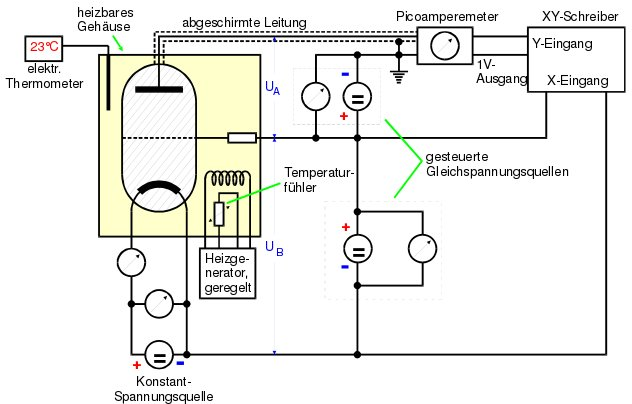
\includegraphics[width=0.7\textwidth]{pics/aufbau_detail.jpeg}
\caption{Verwendeter Aufbau inklusive X-Y-Schreiber$^{[1]}$}
\end{figure}
\section{Durchführung}
Zunächst soll die integrale Energieverteilung der Elektronen bestimmt werden. Man stellt dazu die Beschleunigungsspannung $U_B$ auf konstante 11V ein und lässt den X-Y-Schreiber dann den Auffängerstrom gegen die Gegenspannung aufzeichnen.

Anschließend soll eine Franck-Hertz-Kurve im Temperaturbereich von 160 - 200$^\circ$ C gezeichnet werden. Hierzu schließt man die Beschleunigungsspannung an den X-Eingang des Schreibers an.

Zum Schluss soll die Ionisierungsspannung von Quecksilber bestimmt werden. Hierzu legt man eine Gegenspannung von -30V an und misst bei einer Temperatur zwischen 100 und 110$^\circ$ C den Auffängerstrom.

\section{Auswertung}
\subsection{Fehlerrechnung}
Da viele für die Auswertung notwendigen Größen fehlerbehaftet sind, ist es wichtig, den Einfluss dieser Fehler auf die ermittelten
Größen herauszufinden. Neben den, von den Messapparaturen verursachten Fehlern, dienen der Mittelwert
\begin{formel}[H]
\begin{equation}
 \bar{x} = \frac1N \sum_{i=1}^{N} x_i,
 \label{eq_mittel}
\end{equation}
\caption*{\small{$\bar{x}$ = Mittelwert, N = Anzahl der Messungen}}
\end{formel}
die Gaußsche Fehlerfortpflanzung
\begin{formel}[H]
\begin{equation}
\Delta G = \sqrt{\sum_{i=1}^{N}\left( \frac{\partial G}{\partial x_i}\cdot \Delta x_i\right)^2},
\label{gauss}
\end{equation}
\caption*{$x_i$ = Variable, $\Delta x_i$ = Fehler der Variable}
\end{formel}
und die Standardabweichung des Mittelwerts
\begin{equation}
 \bar s = \sqrt{\frac{1}{N(N-1)} \sum_{i}^{N} (x_i - \bar{x})^2}.
 \label{eq_standard}
\end{equation}

\subsection{Freie Weglänge}
Die in Abschnitt \ref{sec_dampfdruck} genannte Bedingung für die freie Weglänge $\bar w$ hängt von den im Versuch genutzten Temperaturen
ab und wird gemäß \eqref{eq_weglaenge} und \eqref{eq_sättigungsdruck} errechnet. Das Ergebnis, sowie das Verhältnis zur Beschleunigungsstrecke $a$ sind in Tabelle 
\ref{tab_weglaenge} aufgeführt.

\begin{table}[H]
 \begin{tabular}{c|c|r|r|r}
  Erwähnung	&$T$ in K	&$p_{\text{sät}}$ in mbar&$\bar w$ in cm	&$a/w$ \\
  \hline
\ref{sec_energie}&	301,6	&0,007&	42,160&	2,4\\
\ref{sec_energie}&	424,2&	5,011	&0,058&	1727,9\\
\ref{sec_anregung}&	448,2&	11,938&	0,024&	4116,7\\
\ref{sec_ionisation}&	381,2&	0,805&	0,360&	277,5
 \end{tabular}
\caption{freie Weglänge $\bar w$ zu verschiedenen Temperaturen $T$}
\label{tab_weglaenge}
\end{table}

\subsection{Energieverteilung und Kontaktpotenzial}
\label{sec_energie}
Für die Messung bei Raumtemperatur für $T$ = 28,4 $^\circ$C und konstanter Beschleunigungsspannung $U_B$ = 11 V ergibt sich Graphik 
\ref{item_28} in Abschnitt \ref{sec_anhang} des XY-Schreibers. Dazu wurde die Auffangstromstärke $I_A$ in Abhängigkeit der zeitlich kontinuierlich verändernden
Bremsspannung $U_A$ gemessen. Zur Ermittlung der Energieverteilung muss diese Kurve numerisch abgeleitet werden. Dies geschieht durch
die Zuweisung von Differenzenquotienten $\Delta y / \Delta x$ zu dem entsprechenden x-Wert, die in Tabelle \ref{tab_energie28} vorgenommen worden ist.
\begin{table}[H]
 \begin{tabular}{c|c|c|c|c}
$x$ in cm & $y$ in cm & $\Delta x$ in cm& $\Delta y$ in cm & $\Delta y / \Delta x$\\
\hline
0,0&	1,000&	-&	-&	- \\
3,0&	0,991&	3,0&	0,009&	0,003\\
6,0&	0,968&	3,0&	0,023&	0,008\\
9,1&	0,925&	3,1&	0,043&	0,014\\
9,5&	0,913&	0,4&	0,013&	0,031\\
10,0&	0,897&	0,5&	0,016&	0,031\\
10,6&	0,878&	0,6&	0,019&	0,032\\
11,5&	0,839&	0,9&	0,039&	0,043\\
11,8&	0,824&	0,3&	0,015&	0,050\\
12,3&	0,791&	0,5&	0,033&	0,066\\
12,5&	0,776&	0,2&	0,015&	0,075\\
12,7&	0,758&	0,2&	0,018&	0,091\\
13,0&	0,729&	0,3&	0,028&	0,094\\
13,3&	0,694&	0,3&	0,035&	0,117\\
13,6&	0,647&	0,3&	0,048&	0,158\\
13,8&	0,603&	0,2&	0,044&	0,219\\
14,0&	0,553&	0,2&	0,050&	0,250\\
14,3&	0,400&	0,3&	0,153&	0,510\\
14,6&	0,150&	0,3&	0,250&	0,833\\
14,9&	0,038&	0,3&	0,113&	0,375\\
15,3&	0,011&	0,4&	0,026&	0,066\\
15,6&	0,006&	0,3&	0,005&	0,017\\
 \end{tabular}
\caption{Aus Graphik \ref{item_28} ausgesuchte Wertepaare zur Erstellung von Abbildung \ref{pic_energie28}}
\label{tab_energie28}
\end{table}
Hieraus ergibt sich Abbildung \ref{pic_energie28}. Die negative numerische Ableitung dient lediglich der Übersichtlichkeit.
\begin{figure}[H]
 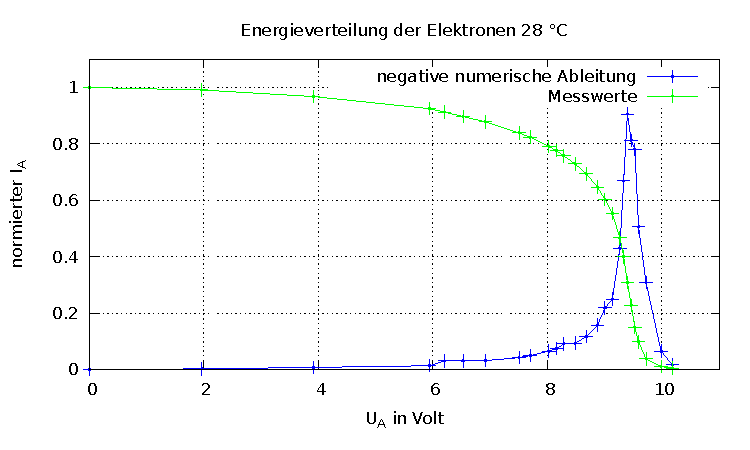
\includegraphics[width=0.8 \textwidth]{pics/energie28.pdf}
 \caption{Auffangstromstärke $I_A$ gegen Bremsspannung $U_A$ bei 28,4 $^{\circ}$C und die negative, numerische Ableitung}
 \label{pic_energie28}
\end{figure}
Es ist hier deutlich festzustellen, dass die Elektronen größtenteils eine hohe, einheitliche Energie aufweisen. Der Peak liegt beim
x-Wert $x$ = 14,6 cm, was nach Tabelle \ref{tab_umrech28} zu einer Spannung führt von
\begin{align}
 U_{A,max} = 9,53 \pm 0,04 \, \text{V}.
\end{align}

\begin{table}[H]
 \begin{tabular}{c|c|c}
  $x$ in cm & $U$ in V & $U/x$ in V/m\\
  \hline
9,1 &	6&	0,66 \\
10,6&	7&	0,66\\
12,3&	8&	0,65\\
13,8&	9&	0,65\\
15,6&	10&	0,64\\
\hline
&	$\langle \frac{U}{x} \rangle$ &	0,65$\pm$0,003
 \end{tabular}
\caption{Umrechnung von $x$ zu $U$}
\label{tab_umrech28}
\end{table}
Der Spannungswert entspricht den Erwartungen, da er etwas geringer als die Beschleunigungsspannung $U_B$ ist. Das nun zu errechnende Kontaktpotenzial
$K$ ergibt sich zu
\begin{align}
 K = U_B - U_{A,max} = 1,47 \pm 0,01 \, \text{V}.
\end{align}

Bei Erhöhung der Betriebstemperatur auf 151 $^\circ$C ergibt sich Graphik \ref{item_151} und die zugehörige Abbildung \ref{pic_energie151}
analog zur eben geschilderten Methode. Die zugehörigen Wertepaare sind in Tabelle \ref{tab_energie151} zu finden.

\begin{table}[H]
 \begin{tabular}{c|c|c|c|c}
$x$ in cm & $y$ in cm & $\Delta x$ in cm& $\Delta y$ in cm & $\Delta y / \Delta x$\\
\hline
0,0&	1,000&	-&	-&	- \\
1,0&	0,865&	1,0&	0,135&	0,135\\
1,8&	0,773&	0,8&	0,092&	0,115\\
2,5&	0,696&	0,7&	0,077&	0,110\\
3,0&	0,633&	0,5&	0,063&	0,126\\
3,6&	0,562&	0,6&	0,072&	0,119\\
4,0&	0,512&	0,4&	0,050&	0,125\\
4,5&	0,448&	0,5&	0,064&	0,128\\
5,0&	0,388&	0,5&	0,059&	0,118\\
5,5&	0,331&	0,5&	0,058&	0,115\\
6,0&	0,275&	0,5&	0,056&	0,112\\
6,5&	0,223&	0,5&	0,052&	0,103\\
7,0&	0,172&	0,5&	0,051&	0,102\\
7,3&	0,145&	0,3&	0,028&	0,092\\
7,5&	0,128&	0,2&	0,016&	0,081\\
8,0&	0,096&	0,5&	0,032&	0,065\\
8,3&	0,077&	0,3&	0,019&	0,064\\
8,6&	0,065&	0,3&	0,012&	0,038\\
9,0&	0,058&	0,4&	0,008&	0,019\\
9,5&	0,054&	0,5&	0,004&	0,008\\
10,0&	0,052&	0,5&	0,002&	0,003\\
10,6&	0,048&	0,6&	0,005&	0,008\\
11,0&	0,046&	0,4&	0,002&	0,004
 \end{tabular}
\caption{Aus Graphik \ref{item_151} ausgesuchte Wertepaare zur Erstellung von Abbildung \ref{pic_energie151}}
\label{tab_energie151}
\end{table}

Die Umrechnung von $x$ zu $U$ wird nach Tabelle \ref{tab_umrech151} vorgenommen
\begin{table}[H]
 \begin{tabular}{c|c|c}
$x$ in cm & $U$ in V & $U/x$ in V/m\\
\hline
1,8&	1&	0,56 \\
3,6&	2&	0,56\\
5,5&	3&	0,55\\
7,3&	4&	0,55\\
9,0&	5&	0,56\\
10,6&	6&	0,57\\
&$\langle \frac{U}{x} \rangle$	&	0,55 $\pm$ 0,003
 \end{tabular}
\caption{Umrechnung von $x$ zu $U$}
\label{tab_umrech151}
\end{table}

\begin{figure}[H]
 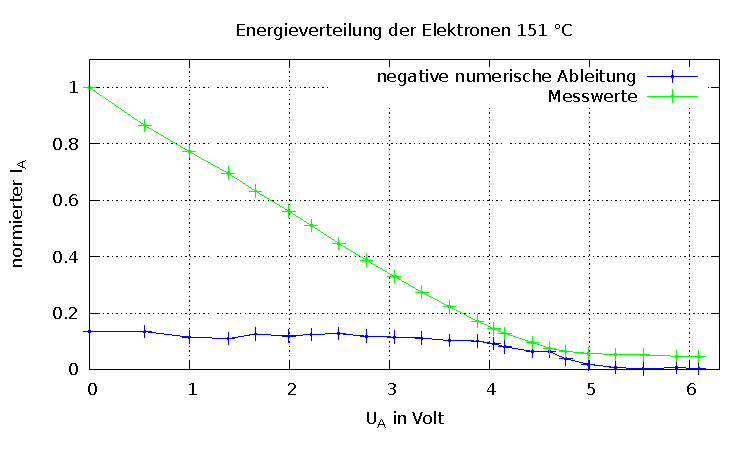
\includegraphics[width=0.8 \textwidth]{pics/energie151.pdf}
 \caption{Auffangstromstärke $I_A$ gegen Bremsspannung $U_A$ bei 151 $^{\circ}$C und die negative, numerische Ableitung}
 \label{pic_energie151}
\end{figure}

Es ist leicht zu erkennen, dass die Energieverteilung der Elektronen bei höherer Temperatur deutlich breiter ist. Daher ist hiermit
das Kontaktpotenzial nicht bestimmbar.

\subsection{Anregungsenergie des Quecksilberatoms}
\label{sec_anregung}
Zur Bestimmung der Anregungsenergie des Quecksilberatoms wird eine Franck-Hertz-Kurve bei einer Temperatur von 175 $^{\circ}$C erstellt.
Hierzu wird bei einer konstanten Bremsspannung von $U_A$ = 1 V die Beschleunigungsspannung $U_B$ kontinuierlich erhöht und dazu die
Auffangstromstärke gemessen. In Graphik \ref{item_franck} ist der Verlauf zu sehen. Die Maxima des Graphen werden den jeweiligen Spannungen in
Tabelle \ref{tab_franck} zugewiesen und ihre Differenzen angegeben. 
\begin{table}[H]
 \begin{tabular}{c|r|r|r}
Maximum& $x$ in cm &	$U_B$ in V&	$\Delta U$ in V\\
\hline
1& 	2,46& 	6,51& -	\\
2& 	4,25	& 11,25&	4,74 \\
3& 	6,07&	16,07&	4,82\\
4& 	7,94&	21,02&	4,95\\
5& 	9,87&	26,13&	5,11\\
6& 	11,79&  31,21&	5,08\\
7& 	13,90& 	36,50&	5,29
 \end{tabular}
\caption{Beschleunigungsspannung $U_B$ für die jeweiligen Maxima der Franck-Hertz-Kurve, sowie Spannungsdifferenzen der Maxima zueinander}
\label{tab_franck}
\end{table}
Somit ergibt sich ein gemittelter Wert für die Spannungsdifferenz bzw. der Anregungsenergie
\begin{align}
 e \cdot \langle \Delta U \rangle= \Delta E = 5,00 \pm 0,08 \, \text{eV}.
\end{align}
Die daraus resultierende Wellenlänge für das emittierte Photon ergibt sich aus \eqref{eq_energie_phtoton} zu
\begin{align}
 \lambda = 248,2 \pm 4,1 \, \text{nm}.
\end{align}
Der Energieverlust der Elektronen beim zentralen, elastischen Stoß nimmt mit zunehmender Temperatur zu, jedoch ist der Einfluss kaum
zu beachten, da der relative Fehler der Anregungsenergie sehr klein ist, im Gegensatz zu Ablesefehlern.

\subsection{Ionisationsspannung von Quecksilber}
\label{sec_ionisation}
Zur Ermittlung der Ionisationsspannung von Quecksilber $U_{ion}$ wird bei einer konstanten Bremsspannung von $U_A$ = 30 V die Auffangstromstärke
bei zeitlich, kontinuierlich verändernden Beschleunigungsspannung $U_B$ gemessen. Graphik \ref{item_ion} zeigt den Verlauf bei einer
Betriebstemperatur von 108 $^{\circ}$C. Der Spannungswert für $U_B$, bei dem der Graph nur noch linear steigt, gibt die Ionisationsspannung
für Quecksilber an, wobei nach Abschnitt \ref{sec_kontakt} mit \eqref{eq_ionisation} dieser Wert noch um das Kontaktpotenzial $K$ verschoben
werden muss. So ergibt sich
\begin{align}
 e \cdot U_{ion} = E_{ion} = 12,72 \, \text{eV} - 1,47 \, \text{eV} = 10,98 \pm 0,07 \, \text{eV}.
\end{align}


\section{Diskussion}
Der Wert für die freie Weglänge $\bar w$ spielt lediglich für die Auswertung der Franck-Hertz-Kurve eine Rolle. So liegt ihr Wert von
$\bar w$ = 0,24 mm bzw. das Verhältnis $a/\bar w$ = 4116 knapp über dem Bereich von 1000 bis 4000, der in Abschnitt \ref{sec_dampfdruck} 
gefordert ist, jedoch ist dies nicht weiter problematisch.

Der Unterschied der beiden Energieverteilungen in Abschnitt \ref{sec_energie} ist sehr gut erkennbar. Aufgrund der relativ geringen
Temperatur von 28,4 $^\circ$C für Graphik \ref{item_28} haben die Elektronen zu Beginn eine einigermaßen einheitliche Anfangsgeschwindigkeit.
Daher erhalten sie auf ihrem Weg weitgehend dieselbe Energiezufuhr, weshalb abzüglich des Kontaktpotenzials kein Elektron die Auffangelektrode
mehr erreicht. Über die Güte der Auswertung für das Kontaktpotenzial können keine Aussagen getroffen werden, da die verwandten Materialen
nicht bekannt sind.

Der Graphik \ref{item_franck} lassen sich die Maxima sehr gut entnehmen. Unter fehlender Berücksichtigung entstehender Ablesefehler kann
der ermittelte Wert $\Delta E$ = 5,00 eV gut mit dem Referenzwert$^{[2]}$ mit $\Delta E_{ref}$ = 4,9 eV verglichen werden
\begin{align}
 \frac{\Delta E}{\Delta E_{ref}} - 1 = 2,0\,\%.
\end{align}

Etwas schwierig bei der Ermittlung von $U_{ion}$ ist die hohe Ableseungenauigkeit. Die Normierung der x-Achse auf Volt hat hierbei
einen bis zu vierfach höheren Wert, als bei den anderen Auswertungsabschnitten. Jedoch ist hier ebenfalls der ermittelte Wert von
$E_{ion}$ = 10,98 eV durchaus annehmbar. Verglichen mit dem Referenzwert$^{[3]}$ $E_{ion,ref}$ = 10,44 eV ergibt sich eine Abweichung von
\begin{align}
 \frac{E_{ion}}{E_{ion,ref}}-1 = 5,2 \,\%.
\end{align}



\section{Anhang}
\label{sec_anhang}
\begin{enumerate}
 \item Energieverteilung bei 28,4 $^\circ$C
 \label{item_28}
 \item Energieverteilung bei 151 $^\circ$C
 \label{item_151}
 \item Franck-Hertz-Kurve bei 175 $^{\circ}$C 
 \label{item_franck}
 \item Ionisationsspannung bei 108 $^{\circ}$C
 \label{item_ion}
\end{enumerate}

 



% ========================================
%	Literaturverzeichnis
% ========================================

%\bibliographystyle{plainnat}			% Bibliographie-Style auswählen
%\bibliography{BIBDATEI}			% Literaturverzeichnis
\parskip 200pt
\Large{Literatur}\\\\
\large{[1] Versuchsanleitung - Der Franck-Hertz-Versuch}\\\\
\large{[2] Dr. Maxton-Küchenmeister J., \textit{Atomarer Energieaustausch | LEIFI Physik}, \\URL: \href{http://www.leifiphysik.de/themenbereiche/atomarer-energieaustausch/geschichte#Franck-Hertz\%20-\%20Historisches}{www.leifiphysik.de/themenbereiche/atomarer-energieaustausch}}\\\\
\large{[3] Hoppe A., \textit{Quecksilber - Atomeigenschaften}, \\URL: \href{http://www.periodensystem.info/elemente/quecksilber/}{www.periodensystem.info/elemente/quecksilber/}}\\\\

\end{document}

% ========================================
%	Das Dokument endent
% ========================================

\end{document}
